\documentclass{report}
\usepackage{etoolbox}
\usepackage{graphicx}
\usepackage{amsmath}
\usepackage{ragged2e}  % Pacchetto per l'allineamento del testo
\usepackage{color}   %May be necessary if you want to color links
\usepackage{hyperref}
\usepackage{outlines}
\usepackage{enumitem}


\hypersetup{
    colorlinks=true, %set true if you want colored links
    linktoc=all,     %set to all if you want both sections and subsections linked
    linkcolor=black,  %choose some color if you want links to stand out
}

\newcounter{myexample}[chapter]  % Numerazione con il numero di sezione
\renewcommand{\themyexample}{\arabic{chapter}.\arabic{myexample}}  % Formato del contatore

\newenvironment{myexample}[1][]{
  \refstepcounter{myexample}
  \par\medskip\noindent{\itshape Esempio \themyexample\quad #1} \ignorespaces
}{
  \par\medskip
}


\newcounter{myobservation}[chapter]  % Numerazione con il numero di sezione
\renewcommand{\themyobservation}{\arabic{chapter}.\arabic{myobservation}}  % Formato del contatore

\newenvironment{myobservation}[1][]{
  \refstepcounter{myobservation}
  \par\medskip\noindent\textbf{Osservazione \themyobservation\quad #1} \ignorespaces
}{  \par\medskip
}

\newcounter{myintuition}[chapter]  % Numerazione con il numero di sezione
\renewcommand{\themyintuition}{\arabic{chapter}.\arabic{myintuition}}  % Formato del contatore

\newenvironment{myintuition}[1][]{
  \refstepcounter{myintuition}
  \par\medskip\noindent\textbf{Intuizione \themyintuition\quad #1} \ignorespaces
}{  \par\medskip
}

\newcounter{mydefinition}[chapter]  % Numerazione con il numero di sezione
\renewcommand{\themydefinition}{\arabic{chapter}.\arabic{mydefinition}}  % Formato del contatore

\newenvironment{mydefinition}[1][]{
  \refstepcounter{mydefinition}
  \par\medskip\noindent\textbf{Definizione \themydefinition\quad #1} \ignorespaces
}{  \par\medskip
}

\newcounter{mytheorem}[chapter]  % Numerazione con il numero di sezione
\renewcommand{\themytheorem}{\arabic{chapter}.\arabic{mytheorem}}  % Formato del contatore

\newenvironment{mytheorem}[1][]{
  \refstepcounter{mytheorem}
  \par\medskip\noindent\textbf{Teorema \themytheorem\quad #1} \ignorespaces
}{  \par\medskip
}

\newcounter{mynotation}[chapter]  % Numerazione con il numero di sezione
\renewcommand{\themynotation}{\arabic{chapter}.\arabic{mynotation}}  % Formato del contatore

\newenvironment{mynotation}[1][]{
  \refstepcounter{mynotation}
  \par\medskip\noindent\textbf{Notazione \themynotation\quad #1} \ignorespaces
}{  \par\medskip
}


\newcounter{myexercise}[chapter]  % Numerazione con il numero di sezione
\renewcommand{\themyexercise}{\arabic{chapter}.\arabic{myexercise}}  % Formato del contatore

\newenvironment{myexercise}[1][]{
  \refstepcounter{myexercise}
  \par\medskip\noindent\textbf{Esercizio \themyexercise\quad #1} \ignorespaces
}{  \par\medskip
}

\newcounter{myimage}[chapter]
\renewcommand{\themyimage}{\thechapter.\arabic{myimage}}

\begin{document}
\begin{titlepage}
    \title{Traduzione Handout Giunchilgia}

\author{
    Nicolas Torriglia\\
    \and
    Chat GPT\\
}
\date{}

\maketitle
\end{titlepage}


\newpage



\cleardoublepage
\setcounter{page}{2}
\tableofcontents

\chapter{Il mondo e la mente}
\section{Frames della mente} 
\section{Illusioni ottiche}
\section{Fallacie mentali}
\section{Quindi?}

\chapter{Rappresentazioni}
\section{Il gap semantico}
\section{Rappresentazioni mentali}
\section{Rappresentazioni}
\section{Esercizi}

\chapter{Modelli e teorie asserzionali}
L'osservazione 2.15 potrebbe suggerire che non esista una soluzione al problema della soggettività delle rappresentazioni mentali. Tuttavia, ciò non è vero. L'osservazione chiave è che le rappresentazioni sono costruite dagli esseri umani con lo scopo specifico di far convergere il più possibile le rappresentazioni mentali della stessa rappresentazione, minimizzando in particolare la probabilità di incongruenze. La domanda da affrontare è come costruire tali rappresentazioni.
\section{Modelli}
Il punto di partenza sono le rappresentazioni mentali analogiche, poiché le nostre rappresentazioni hanno inizio da qui. Considera l'esempio seguente.
\begin{myexample}[(Cosa c'è in una rappresentazione analogica)]
    Considera la rappresentazione analogica illustrata nell'immagine della Figura 3.1. Possiamo vedere tre persone, che possiamo assumere abbiano i nomi Paolo, Stefania e Sofia, che sono amici, vari cani, il fatto che siano uno a destra dell'altro e, naturalmente, molto altro.    
\end{myexample}
\clearpage
\begin{figure}[ht]
    \centering
    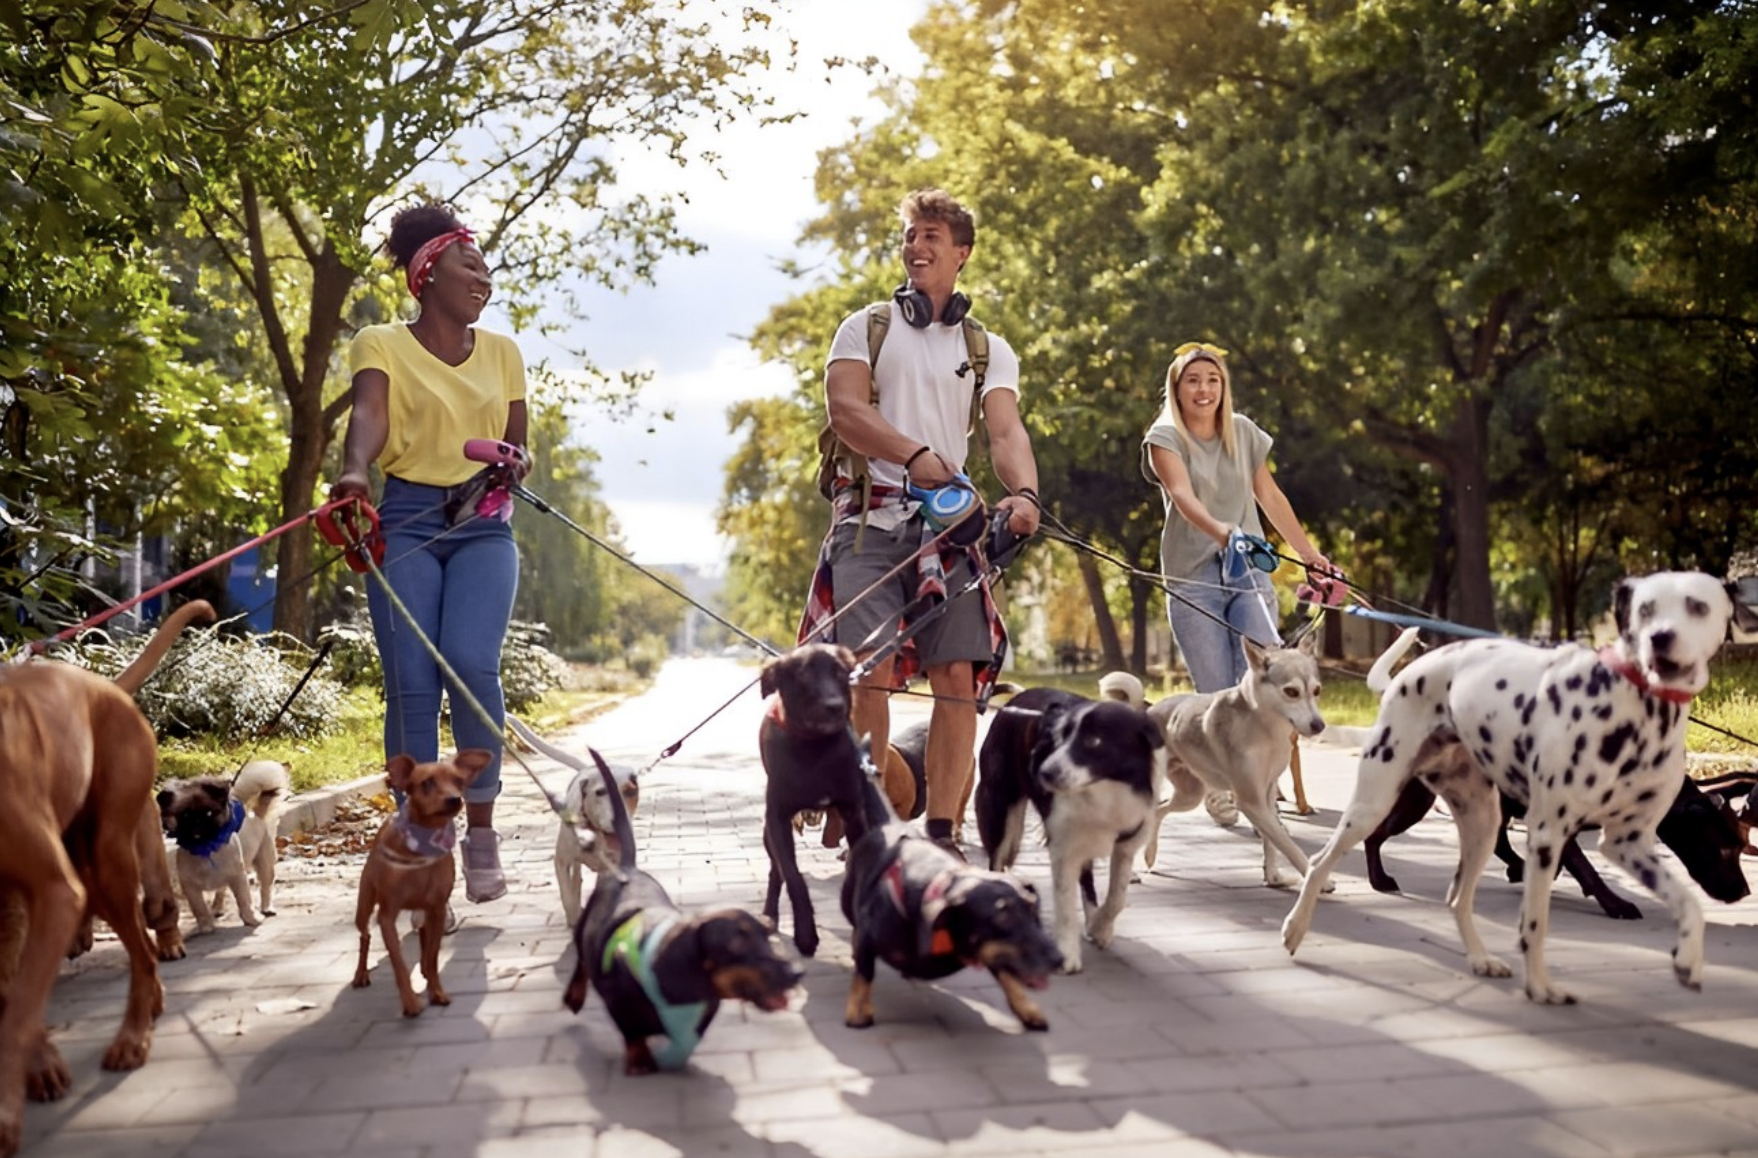
\includegraphics[width=0.7\linewidth]{imgs/img3.1.png}
    \caption{Una rappresentazione analogica di una situazione quotidiana}
\end{figure}

\begin{myobservation}[(Cosa c'è in una rappresentazione analogica)]
    Considera la rappresentazione analogica illustrata nell'immagine della Figura 3.1. Possiamo vedere tre persone, che possiamo assumere abbiano i nomi Paolo, Stefania e Sofia, che sono amici, vari cani, il fatto che siano uno a destra dell'altro e, naturalmente, molto altro.    
\end{myobservation}

\begin{myintuition}[(Fatto)]
    Un fatto \verb+f+ è un qualcosa che succede certamente ad una certa coordinata spaziotemporale
\end{myintuition}

\begin{mydefinition}[(Modello)]
    Un modello \verb+M+ è un set di fatti \verb+F = {f}+
    \begin{equation}
        \verb+M = {f}+
    \end{equation}
\end{mydefinition}

\begin{myobservation}[(Fatti e modelli)] I fatti sono gli elementi atomici, non ulteriormente decomponibili, di un modello. Nota che, a differenza dei modelli, i fatti sono considerati come una nozione primitiva e quindi non possono essere definiti formalmente.
\end{myobservation}

\begin{myexample}[(I fatti di un modello rappresentato nella Figura 3.1)]
    Un modello, uno tra molti altri, della situazione rappresentata nella Figura 3.1 potrebbe contenere, ad esempio, i seguenti fatti:
    \begin{verbatim}
    Sofia è una persona         Paolo è un uomo
    Rocky è un cane             Sofia è vicina a Paolo
    Sofia ha i capelli biondi   Sofia è un'amica di Paolo
    Rocky è un animale          Rocky è il cane di Sofia
    \end{verbatim}
\end{myexample}

\begin{myobservation}[(La soggettività dei fatti)]
    I fatti sono ciò che viene osservato e anche descritto, ad esempio, a terze persone. Il problema è che, proprio a causa di quanto discusso nella Sezione 2.2 e, nello specifico, il fatto di cosa siano i fatti è soggettivo e nascosto nelle menti delle persone che li percepiscono. Quanti altri fatti più e/o diversi da quelli elencati nell'Esempio 3.2 potresti immaginare? Potrebbero essere infiniti! Nota che ogni fatto può essere decomposto in qualsiasi insieme di fatti più semplici se questo è l'attuale focus dell'osservatore. Quindi, per esempio, anziché concentrarsi su Sofia, potrei concentrarmi sui suoi capelli, sulle sue gambe o su...
\end{myobservation}

\begin{myobservation}[(Fatti mutualmente (in)coerenti in un modello)]
    Il modello dell'Esempio 3.2 potrebbe essere esteso per affermare il fatto che Sofia è una donna o che Paolo è una persona. Tuttavia, avremmo problemi nell'estenderlo aggiungendo il fatto che Paolo è una donna o che Sofia è un cane, poiché avremmo due fatti mutualmente inconsistenti, qualcosa che sappiamo non può accadere nel mondo come lo percepiamo. Vedi anche l'Osservazione 2.9. Un modello non può contenere fatti che, almeno intuitivamente, sono mutualmente inconsistenti. Oltre a questo semplice esempio, la questione è come formalizzare questa intuizione e quindi come essere in grado di rilevarla mediante il ragionamento sui modelli.
\end{myobservation}

\begin{myobservation}[(Fatti e affermazioni)]
    Per essere considerato un fatto, deve essere descritto linguisticamente come tale. Non è per caso che nell'Esempio 3.2 abbiamo indicato i fatti attraverso un insieme di descrizioni in linguaggio naturale. Chiamiamo tali descrizioni "affermazioni". Il modo più semplice di pensare a un'affermazione è come a una frase dichiarativa in linguaggio naturale articolata in termini di un soggetto che si trova in una relazione più o meno complessa con un oggetto (come ad esempio, "Stefania sta camminando con i cani verso il centro della città"), o di un soggetto che detiene.
\end{myobservation}


\section{Teorie asserzionali}
\begin{myobservation}[(Affermazioni e teorie assertive)]
    Le affermazioni sono descrizioni indivisibili, diciamo atomiche, di un fatto. Le teorie assertive sono descrizioni di modelli.
\end{myobservation}

\begin{myintuition}[(Affermazione)]
    Un'affermazione $a$ è una rappresentazione linguistica atomica di un certo fatto \verb+f+.
\end{myintuition}

\begin{mydefinition}[(Teoria assertiva)]
    Una teoria assertiva $\mathcal{T}_A$ è un insieme di affermazioni.
    \begin{equation}
        \mathcal{T}_A = \{a\}
    \end{equation}

Abbiamo bisogno di definire che un'affermazione è la descrizione di un fatto specifico e, più in generale, che una teoria assertiva descrive un modello.

\begin{myexample}[(Una teoria assertiva del modello rappresentato nella Figura 3.1)]
    Una teoria assertiva, una tra molte altre, che descrive i fatti dell'Esempio 3.2 in linguaggio naturale potrebbe essere, ad esempio:
    \begin{verbatim}
    Sofia è una persona         Paolo è un uomo
    Sofia è vicina a Paolo      Rocky è il cane di Sofia
    Sofia è un’amica di Paolo   Sofia ha i capelli biondi
    Rocky è un cane             Rocky è un animale
    \end{verbatim}

\end{myexample}

Come si può notare, la teoria assertiva è in italiano, poiché essendo in linguaggio naturale può essere espressa anche in questo modo, e potrebbe essere altrettanto espressa in inglese.

\end{mydefinition}

\section{Funzioni d'interpretazione}
\begin{mydefinition}[(Funzione d'interpretazione)]
    Sia $\mathcal{I}_A$ una funzione di interpretazione di una teoria assertiva, definita come:
    \begin{equation}
        \mathcal{I}_A : \mathcal{T}_A \rightarrow \verb|M|
    \end{equation}
    Diciamo che un fatto \verb+f+ $\in$ \verb+M+ è l'interpretazione di $a \in \mathcal{I}_A$, e scriviamo:
    \begin{equation}
        \verb|f| = \mathcal{I}_A(a) = a^{\mathcal{I_A}}
    \end{equation}
    per intendere che $a$ è una descrizione linguistica di \verb|f|. Diciamo che \verb|f| è l'interpretazione di $a$, o, equivalentemente, che a denota \verb|f|.
(Più asserzioni possono portare ad un fatto)
\end{mydefinition}

\begin{myobservation}[(Funzione di interpretazione, polisemia)]
    Si assume che $\mathcal{I}_A$ sia una funzione, ovvero per ogni fatto esiste solo un'affermazione che lo descrive. In effetti, dobbiamo garantire che se due fatti $f_1$ e $f_2$ 
    sono diversi, allora non possono entrambi essere il risultato dell'interpretazione della stessa affermazione $a$, ovvero non può essere che se $\mathcal{T}_A = f_1$ allora anche $\mathcal{T}_A = f_2$. 
    Questo fenomeno, chiamato polisemia, è diffuso nelle lingue naturali ed è una delle principali fonti di malintesi e, di conseguenza, di costruzione di rappresentazioni mentali divergenti della stessa rappresentazione. 
    La polisemia delle affermazioni deriva direttamente dalla polisemia delle parole. Ad esempio: il nome proprio Java ha tre significati, è un linguaggio di programmazione, un tipo di chicchi di caffè e un'isola. La parola "auto" ha vari significati, ad esempio può significare automobile o una parte di un treno. 
    Parole generali, come "fare", hanno più di dieci significati. La polisemia è comune alla maggior parte delle parole, in particolare con quelle parole che vengono più comunemente utilizzate (le persone tendono a dare alle parole il proprio significato specifico) ed è una delle principali complicazioni (se non l'unica) che sorgono durante la costruzione di sistemi di comprensione del linguaggio naturale.
\end{myobservation}

\begin{myobservation}[(La non ambiguità delle funzioni di interpretazione)]
    Come dalla Sezione 1.3, le descrizioni linguistiche sono ambigue. Come dall'Osservazione 3.7, una delle principali ragioni è la polisemia delle parole. Tuttavia, questa ambiguità è nella mente dell'ascoltatore/lettore. Si può assumere che chi parla/scrive abbia sempre in mente l'analoga rappresentazione unica che sta descrivendo. La nozione di funzione di interpretazione impone questa supposizione, obbligando chi parla/scrive a essere esplicito sul significato inteso.
\end{myobservation}

\begin{myobservation}[(Funzione di interpretazione, sinonimia)]
    Due affermazioni sono sinonimi quando hanno lo stesso significato, ovvero l'interpretazione di due affermazioni diverse 
    $a_1$ e $a:$ può denotare lo stesso fatto $f$, ovvero $\mathcal{I}_A(a_1) = I_A(a_2) = f$. Le parole sinonime sono nuovamente diffuse nelle lingue naturali, in particolare con le entità più comuni. Le persone e le entità in generale hanno più nomi, ad esempio nome, cognome, nome più cognome, soprannomi, che sono sinonimi. Diverse lingue generano diversi nomi per la stessa entità (ad esempio, Gran Bretagna, Great Britain). Ci sono anche sostantivi sinonimi, ad esempio auto e automobile. Nota come la parola "auto" sia sia polisemica che sinonima. Anche questo è abbastanza comune. In generale, la sinonimia non è un problema. Tuttavia, nei database relazionali, la sinonimia non è consentita, essenzialmente per motivi di efficienza. I database sono sviluppati sulla base dell'assunzione del nome unico, ovvero nei database, stringhe e affermazioni diverse significano sempre cose diverse.
\end{myobservation}

\begin{myexample}[(Una funzione di interpretazione che fornisce un'interpretazione della teoria assertiva che descrive la Figura 3.1)]
    La funzione di interpretazione naturale che interpreta le frasi nell'Esempio 3.3 (sinistra) nei fatti dell'Esempio 3.2 (destra) è la seguente:
    \begin{FlushLeft}
        \hspace{1cm}
        \parbox{\dimexpr\linewidth-1cm}{
            $\mathcal{I}_A$(Sofia è una persona) = Sofia is a person \linebreak
            $\mathcal{I}_A$(Paolo è un uomo) = Paolo è un uomo \linebreak
            $\mathcal{I}_A$(Rocky è un cane) = Rocky è un cane \linebreak
            ...
            }

    \end{FlushLeft}
\end{myexample}

\begin{myobservation}[(Affermazioni e fatti, soggettività)]
    Il problema della soggettività delle rappresentazioni rimane, essendo un fatto inevitabile della vita. Tuttavia, le nozioni di fatto, affermazione e funzione di interpretazione forniscono uno strumento. In primo luogo, si assume che i fatti siano descritti in modo inequivocabile, tramite funzioni di interpretazione, dalle affermazioni che, a loro volta, sono rappresentazioni linguistiche e, come tali, possono essere condivise. In secondo luogo, le affermazioni, anche se selezionate soggettivamente dagli esseri umani, si presume siano atomiche, cioè forniscono il livello minimo possibile di dettagli con cui un modello può essere descritto.    
\end{myobservation}
\clearpage
\begin{figure}[ht]
    \centering
    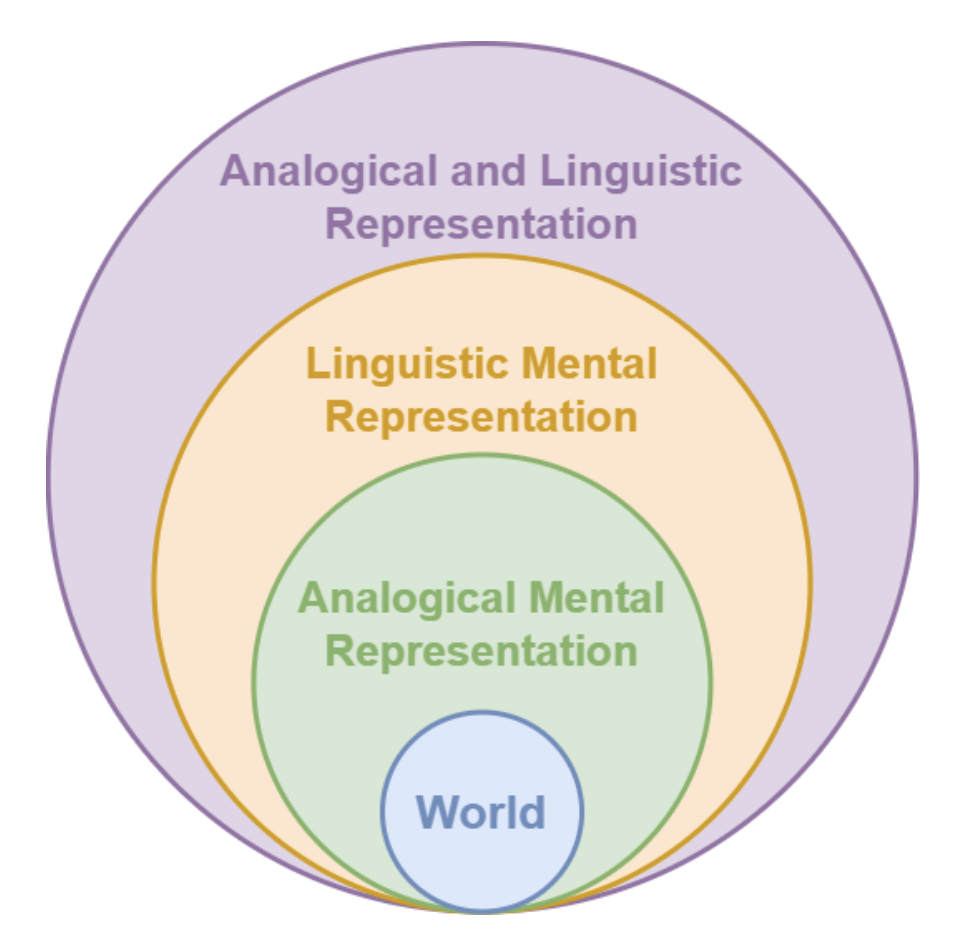
\includegraphics[width=0.7\linewidth]{imgs/img3.2.png}
    \caption{Diagramma di rappresentazione}
\end{figure}

\chapter{Modelli formali e teorie asserzionali}
Per evitare un ragionamento fallace, è necessario rappresentare modelli e teorie assertive in modo inequivocabile, ovvero formale. Quattro sono le caratteristiche che ci interessano:
\begin{itemize}
    \item \textbf{Formalità}: dovrebbe essere un linguaggio logico, ovvero con una sintassi e una semantica ben definite;
    \item \textbf{Universalità}: dovrebbe essere in grado di rappresentare tutti i tipi di fatti;
    \item \textbf{Intuitività}: dovrebbe consentire affermazioni i cui elementi di base (nomi di entità, concetti e proprietà) così come la loro struttura (ovvero come gli elementi di base sono collegati per costruire affermazioni) dovrebbero essere, da un lato, intuitivi per le persone mentre, dall'altro lato, avere una mappatura diretta alla struttura e all'organizzazione del dominio di riferimento;
    \item \textbf{Efficienza} computazionale: $\mathcal{L}_A$ dovrebbe consentire un motore di inferenza veloce ed efficiente, sfruttando l'efficienza intrinseca delle strutture dati utilizzate per memorizzare il modello del mondo.
\end{itemize}

\begin{myobservation}[(Tipi di linguaggi assertivi)]
    I modelli ER e UML sono intuitivi ma non universali, rappresentano solo fatti di conoscenza. I database sono computazionalmente efficienti ma rappresentano solo fatti di dati. Il linguaggio naturale è universale ma la sua semantica non è formalmente definita e non è computazionalmente efficiente. Quest'ultima debolezza si estende anche a sottoinsiemi ben definiti delle lingue naturali. Come esempio di questo caso, i linguaggi logici sono universali con sintassi e semantica ben definite, ma non sono intuitivi da comprendere e anche computazionalmente inefficienti (vedi anche la Sezione 6.5).    
\end{myobservation}

Nella Sezione 4.1, introduciamo alcune definizioni di base della teoria degli insiemi, utili per definire D, mentre, nella Sezione 4.2, introduciamo alcune definizioni di base della teoria dei grafi utili per definire $\mathcal{L}_A$.


    
\section{Teoria degli insiemi}
\subsection{Definizioni base}
Possiamo definire gli insiemi in due modi:
\begin{itemize}
    \item \textbf{Per elencazione}: L'insieme è descritto elencando tutti i suoi elementi (ad esempio, $A=\{a,e,i,o,u\}$).
    \item \textbf{Per astrazione}: L'insieme è descritto attraverso una proprietà dei suoi elementi (ad esempio, $A=\{x|x \text{è una vocale dell'alfabeto latino}\}$).
\end{itemize}

Abbiamo le seguenti definizioni di base.

\begin{mydefinition}[(Insieme vuoto)]
    $\emptyset$ è l'insieme che non contiene alcun elemento.
\end{mydefinition}

\begin{mydefinition}[(Appartenenza)]
    $a \in A$, l'elemento $a$ appartiene all'insieme $A$.
\end{mydefinition}

\begin{mydefinition}[(Non appartenenza)]
    $a \notin A$, l'elemento $a$ non appartiene all'insieme $A$.
\end{mydefinition}

\begin{mydefinition}[(Uguaglianza)]
    $A = B$, se e solo se $A$ e $B$ contengono gli stessi elementi.
\end{mydefinition}

\begin{mydefinition}[(Disuguaglianza)]
    $A \neq B$, se e solo se non è vero che $A = B$.
\end{mydefinition}

\begin{mydefinition}[(Sottoinsieme)]
    $A \subseteq B$, se e solo se tutti gli elementi in $A$ appartengono anche a $B$.
\end{mydefinition}

\begin{mydefinition}[(Sottoinsieme proprio)]
    $A \subset B$, se e solo $ \subseteq B$ e $A \neq B$.
\end{mydefinition}

\begin{mydefinition}[(Insieme universale)]
    L'insieme universale è l'insieme di tutti gli elementi o membri di tutti gli insiemi correlati e è denotato dalla lettera $\mathcal{U}$
\end{mydefinition}

Utilizziamo i \textbf{diagrammi di Venn} per rappresentare gli insiemi. I diagrammi di Venn consistono in cerchi sovrapposti o intersecati che rappresentano insiemi e le loro relazioni. Ogni cerchio rappresenta un insieme specifico, e l'area in cui i cerchi si sovrappongono rappresenta gli elementi condivisi tra gli insiemi corrispondenti. Un elemento che non appartiene a un insieme è rappresentato come un punto al di fuori del cerchio che rappresenta l'insieme.

\begin{mydefinition}[(Unione)]
    Dati due insiemi $A$ e $B$, l'unione di $A$ e $B$ è definita come l'insieme che contiene gli elementi appartenenti a $A$ o a $B$ o ad entrambi, e viene denotata con $\mathbf{A \cup B}$
\end{mydefinition}

\begin{figure}[ht]
    \centering
    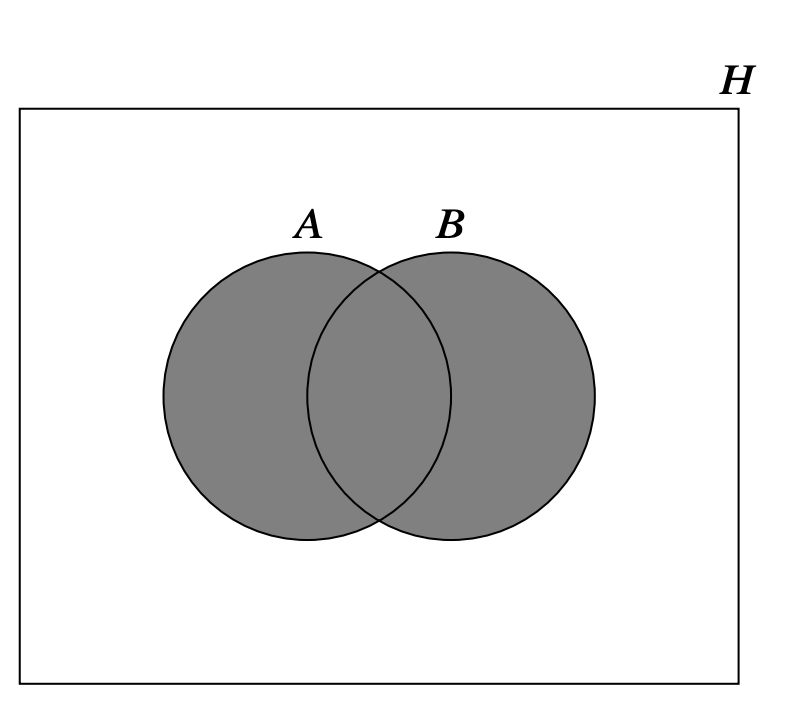
\includegraphics[width=0.3\linewidth]{imgs/img4.1.png}
    \caption{Operazione di unione}
\end{figure}


\begin{mydefinition}[(Intersezione)]
    Dati due insiemi $A$ e $B$, l'intersezione di $A$ e $B$ è definita come l'insieme che contiene gli elementi appartenenti sia a $A$ sia a $B$, e viene denotata con $\mathbf{A \cap B}$
\end{mydefinition}

\begin{figure}[ht]
    \centering
    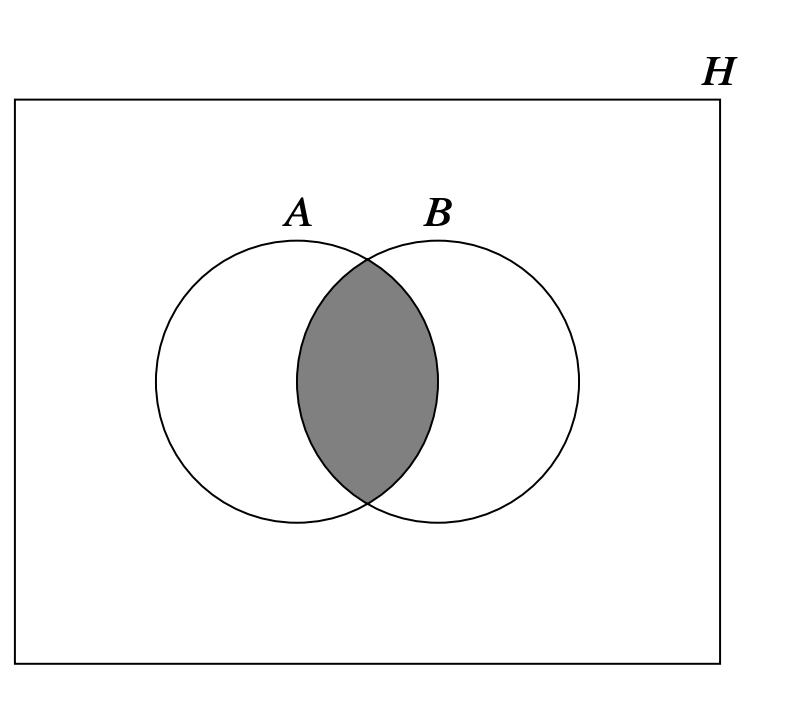
\includegraphics[width=0.3\linewidth]{imgs/img4.2.png}
    \caption{Operazione di intersezione}
\end{figure}


\begin{mydefinition}[(Differenza)]
    La differenza tra due insiemi $A$ e $B$, è definita come l'insieme che contiene gli elementi che sono membri di $A$, ma non membri di $B$. Viene denotata con $\mathbf{A \setminus B}$
\end{mydefinition}

\begin{figure}[ht]
    \centering
    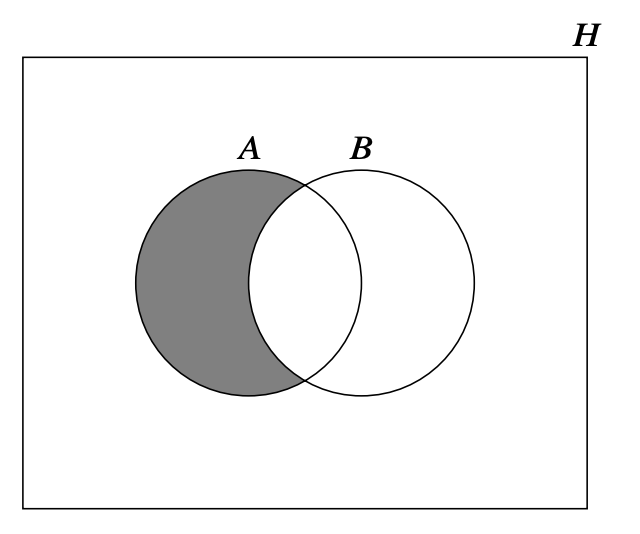
\includegraphics[width=0.3\linewidth]{imgs/img4.3.png}
    \caption{Operazione di differenza}
\end{figure}


\begin{mydefinition}[(Differenza complementare)]
    Dato un insieme universale $U$ e un insieme $A$, dove $A \subseteq U$, il complemento di $A$ in $U$  è definito come l'insieme che contiene tutti gli elementi in $U$ che non appartengono ad $A$ e viene denotato con $\mathbf{A^c}$ o $\mathbf{U \setminus A}$
\end{mydefinition}

\begin{figure}[ht]
    \centering
    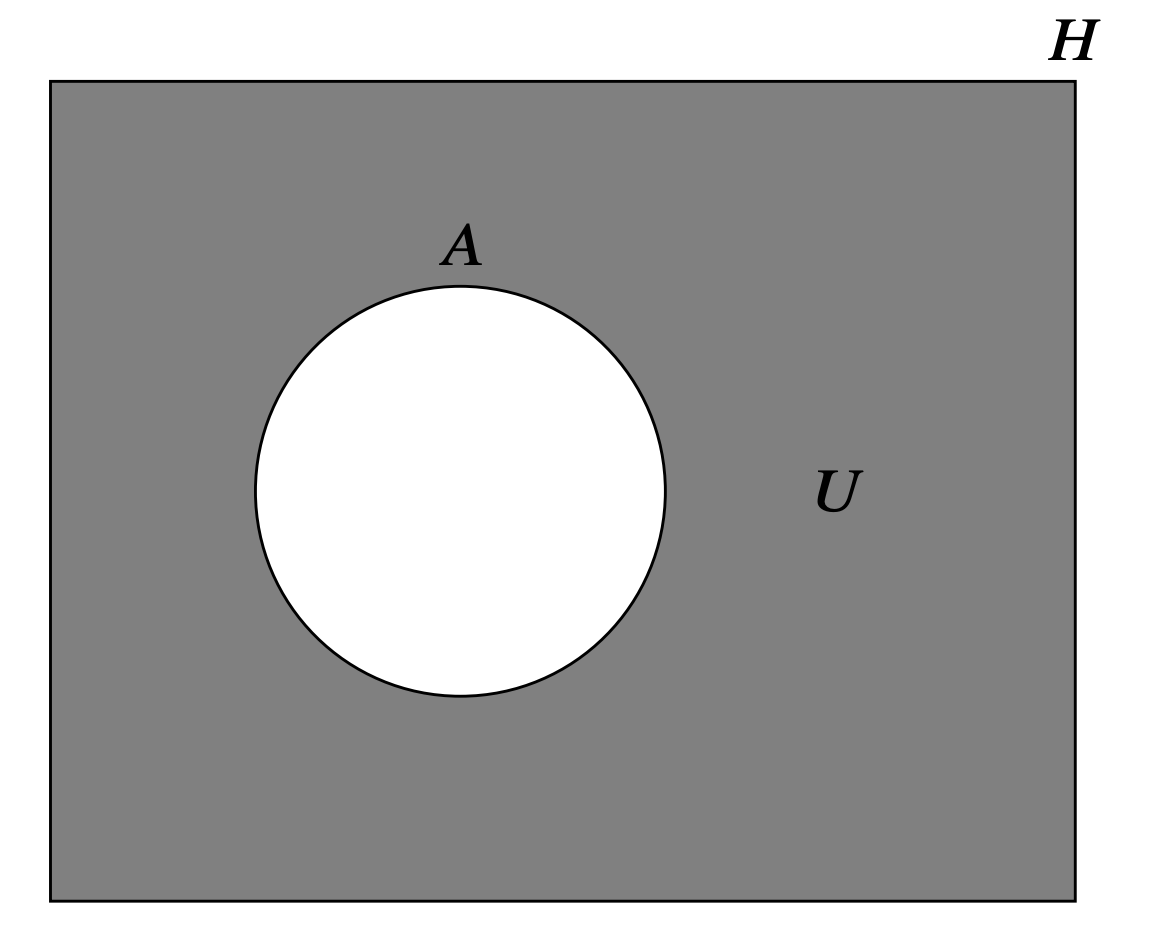
\includegraphics[width=0.3\linewidth]{imgs/img4.4.png}
    \caption{Differenza complementare}
\end{figure}

\begin{mytheorem}[(Proprietà delle operazioni)]
    \begin{outline}
        \1 \textbf{Con lo stesso set}
            \2 $A \cap A = A$
            \2 $A \cup A = A$

        \1 \textbf{Commutativa}
            \2 $A \cap B = B \cap A$
            \2 $A \cup B = B \cup A$

        \1 \textbf{Insieme vuoto}
            \2 $A \cap \emptyset = \emptyset$
            \2 $A \cup \emptyset = A$

        \1 \textbf{Associative}
            \2 $(A \cap B) \cap C = A \cap (B \cap C)$
            \2 $A \cap (B \cup C) = (A \cup B) \cap (A \cup C)$

        \1 \textbf{Leggi di De Morgan}
            \2 $\overline{A \cup B} = \overline{A} \cap \overline{B}$
            \2 $\overline{A \cap B} = \overline{A} \cup \overline{B}$

    \end{outline}
\end{mytheorem}

    \subsection{Relazioni}
    \subsection{Funzioni}
\section{Teorie dei grafi}
    \subsection{Nozioni base}
    \subsection{Grafi ...}
\section{Esercizi}

\chapter{Modello del Mondo - Rappresentazione Estensionale}
Le teorie assertive e i modelli rappresentano un passo importante avanti, ma ci sono ancora tre limitazioni principali:
\begin{itemize}
    \item Stiamo considerando solo i fatti del modello in esame. Cosa succede con i fatti che possono verificarsi negli altri possibili modelli, descrivendo situazioni possibilmente molto diverse?
    \item Il linguaggio utilizzato è molto limitato e consiste solo nell'insieme di affermazioni che descrivono i fatti del modello in esame. Cosa succede alle affermazioni che descrivono fatti in tutti gli altri modelli?
    \item Come conseguenza dei due fatti sopra, la definizione di funzione di interpretazione non è generale. Una nuova e diversa funzione di interpretazione deve essere definita per ogni nuova situazione.
\end{itemize}

\section{Dominio}
Secondo l'Equazione (3.1), un modello \verb|M| è deifinito come \verb|M = {f}|, dove \verb|f| è un insieme di fatti che sono veri in una determinata situazione.
\begin{mydefinition}[Dominio (di interpretazione)]
    Un dominio (di interpretazione) è un insieme di fatti \verb|{f}|
    \begin{equation}
        \verb|D| = \verb|{F}|
    \end{equation}
\end{mydefinition}

\begin{mydefinition}[(Modello)]
    Dato un dominio \verb|D|, un modello \verb|M| è un sott'insieme di \verb|D|
    \begin{equation}
        \verb|M| = \verb|{f}| \subseteq D
    \end{equation}
\end{mydefinition}

\begin{myobservation}[(Dominio, modello)]
    Un dominio è l'insieme di tutti i fatti che siamo disposti a considerare. Un modello è semplicemente il sottoinsieme di fatti che definiamo come rappresentativi di ciò che è il caso nella situazione attuale. La Definizione 5.2 generalizza in modo ovvio la Definizione 3.1.    
\end{myobservation}

\begin{myexample}[(I fatti del dominio rappresentato in Figura 3.1)]
    Un dominio che raccoglie, tra gli altri, i fatti rappresentati nella Figura 3.1 potrebbe contenere, ad esempio, i seguenti fatti:
    \begin{verbatim}
    Sofia is a person       Sofia is a woman
    Paolo is a man          Paolo is a person
    Paolo is a dog          Rocky is a dog
    Sofia is near Paolo     Rocky is the dog of Sofia
    Rocky is the dog of Paolo . . .
    \end{verbatim}
    ... e molti altri
\end{myexample}

\begin{myobservation}[(Dominio)]
    Mentre un modello è l'insieme di fatti che sono veri in una certa situazione, un dominio consiste nell'insieme di fatti che potenzialmente possono essere veri per tutte le possibili situazioni. Un dominio definisce tutto e solo ciò che può essere potenzialmente percepito.
\end{myobservation}

\begin{myobservation}[(Fatti mutuamente inconsistenti in un dominio)]
    Come dall'Esempio 5.1, un dominio, a differenza di un modello, può contenere fatti che, almeno intuitivamente, sono mutuamente inconsistenti. Dato un dominio, ci sono molti modelli potenziali, alcuni dei quali potenzialmente mutuamente inconsistenti. I domini devono consentire la possibile istanziazione di modelli distinti mutuamente inconsistenti, come avviene normalmente nel mondo.
\end{myobservation}


\section{Linguaggio asserzionale}
Secondo l'Equazione (3.2), una teoria assertiva $\mathcal{T}_A$ è definita come $\mathcal{T}_A=\{a\}$, dove $\{a\}$ è un insieme di affermazioni che descrivono i fatti che sono veri in una determinata situazione.

\begin{mydefinition}[(Linguaggio assertivo)]
    Un linguaggio assertivo $mathcal{L}_A$è un insieme di affermazioni $\{a\}$
    \begin{equation}
        \mathcal{L}_A = \{a\}
    \end{equation}
\end{mydefinition}

\begin{mydefinition}[(Teoria asserzionale)]
    Data un linguaggio assertivo $\mathcal{L}_A$, una teoria assertvia $\mathcal{T}_A$ è un sottonsieme di $\mathcal{L}_A$
    \begin{equation}
        \mathcal{T}_A = \{a\} \subseteq \mathcal{L}_A
    \end{equation}
\end{mydefinition}

\begin{myobservation}[(Linguaggio assertivo)]
    Mentre una teoria assertiva è l'insieme di affermazioni che descrive ciò che è vero in un certo modello, un linguaggio assertivo consiste nell'insieme di affermazioni che descrivono tutti i fatti che possono potenzialmente verificarsi. La Definizione 5.4 si estende in modo ovvio dalla Definizione (3.2).
\end{myobservation}

\begin{myexample}[(Linguaggio assertivo)]
    Il linguaggio dell'Esempio 3.3 esteso per includere tutti i fatti del dominio definito nell'Esempio 5.1 allo stesso modo (ossia, traduzioni italiane citate della frase in inglese che descrive un fatto) è un linguaggio assertivo.
\end{myexample}

\begin{myobservation}[(Completezza e correttezza di un linguaggio assertivo $\mathcal{L}_A$ rispetto a un dominio $D$)]
    Un linguaggio assertivo non è necessariamente completo, ovvero non contiene necessariamente affermazioni per tutti i fatti in un dominio (che, tra le altre cose, sono in principio infiniti). La caratteristica chiave è che dovrebbe contenere tutte le affermazioni ritenute rilevanti. Viceversa, un linguaggio assertivo è richiesto di essere corretto, cioè di contenere solo affermazioni che denotano fatti nel dominio di riferimento, al fine di evitare affermazioni prive di senso.
\end{myobservation}

\begin{myexample}[(Linguaggi assertivi):]
    \begin{enumerate}
        \item Linguaggi che consentono solo affermazioni in linguaggio naturale della forma "$<$soggetto$>$ $<$verbo$>$ $<$oggetto$>$" descrivono fatti sul mondo. Il linguaggio utilizzato è una sequenza di affermazioni semplici senza frasi complesse.
        \item I database relazionali (DB) descrivono fatti sul mondo. Il linguaggio utilizzato per descrivere i contenuti di un database relazionale sono le tabelle;
        \item I modelli entity-relationship (ER) descrivono fatti generali sui contenuti dei database. Sono scritti utilizzando il linguaggio del diagramma ER, un linguaggio di grafi specificamente etichettato.
        \end{enumerate}
\end{myexample}

\section{Funzione d'interpretazione}
\begin{mydefinition}[(Funzione di interpretazione)]
    Sia $\mathcal{L}_A$ un linguaggio di asserzioni e \verb|D| un dominio. Quindi, una Funzione di Interpretazione di un linguaggio assertivo $\mathcal{I}_A$ è definita come:

    \begin{equation}
        \mathcal{I}_A : \mathcal{L}_A \rightarrow \verb|D| \quad (\mathcal{I}_A \subseteq \mathcal{L}_A \times \verb|D|)
    \end{equation}

\end{mydefinition}

Vedi 3.3 (ripetizione) ... Andiamo avanti

\section{Modello del mondo}
Il viaggio è completo. Dobbiamo soltanto mettere tutto insieme.

\begin{myobservation}[(I ruoli di D,\(\mathcal{L}, \mathcal{I}_A, M, \mathcal{T}_A\))]
    Le definizioni fornite nelle sezioni precedenti possono essere riassunte dalla seguente figura.
    \begin{equation}
        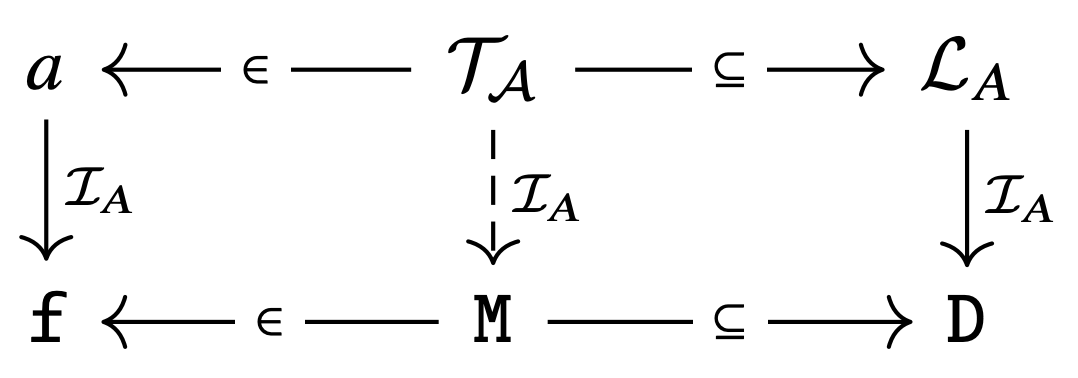
\includegraphics[height=15ex]{imgs/eq5.6.png}
    \end{equation}

\end{myobservation}

Nell'Equazione (5.7), \verb|D| definisce l'insieme di fatti $f$ di potenziale interesse, \verb|M| l'insieme di fatti su cui ci stiamo concentrando, $\mathcal{L}_A$  l'insieme di affermazioni $a$ di potenziale interesse e, infine, $\mathcal{T}_A$ è la teoria che descrive \verb|M|. In altre parole, come singole affermazioni $a$ descrivono singoli fatti f da un lato, e come gli insiemi complessivi di affermazioni $\mathcal{L}_A$ descrivono \verb|D| dall'altro lato, definiscono l'ambito entro il quale una teoria assertiva $\mathcal{T}_A$ può concentrarsi per descrivere modelli specifici \verb|M|. Affermazioni, linguaggi e teorie sono semplicemente i mezzi per specificare il modello desiderato enunciando i fatti desiderati tra quelli consentiti dal dominio di riferimento.
\begin{mydefinition}[(Modello del mondo)]
    \begin{equation}
        \hat{\mathcal{W}} = \langle \mathcal{L}_A, \verb|D|, \mathcal{I}_A \rangle 
    \end{equation}
    è un \textbf{modello del mondo}
\end{mydefinition}

\begin{myobservation}[(Modello del mondo)]
    Nell'Equazione (5.7), i componenti di un modello del mondo, cioè $\mathcal{L}_A, \verb|D|, \mathcal{I}_A$ definiscono le regole generali che vengono seguite durante la costruzione di una rappresentazione. Sono definiti a priori, di solito da esperti di modellizzazione e rappresentazione della conoscenza, come strumenti generali da utilizzare da parte degli operatori. Forniscono l'infrastruttura generale di modellazione che consente di rappresentare problemi del mondo reale. Forniscono anche un quadro uniforme con il quale è possibile confrontare e, eventualmente, anche unire due rappresentazioni. Gli sviluppatori di software di solito studiano questi modelli durante alcuni corsi di informatica o intelligenza artificiale e li utilizzano così come sono nello sviluppo di sistemi; si pensi, ad esempio, all'ampio utilizzo dei modelli ER (Entity-Relationship).
\end{myobservation}

\begin{myobservation}[(Dalle rappresentazioni mentali ai modelli del mondo)]
    I modelli del mondo sono spazi di rappresentazioni possibili, cioè teorie, progettati per minimizzare la possibilità di diverse rappresentazioni mentali della stessa teoria e del corrispondente modello che raffigura il mondo.
\end{myobservation}

I modelli del mondo forniscono il quadro generale entro il quale le teorie assertive e i modelli possono essere definiti e confrontati.

\begin{myobservation}[(Teoria e modello)]
    Ricorda che, dato un modello di un mondo $\hat{\mathcal{W}} = \langle \mathcal{L}_A, \verb|D|, \mathcal{I}_A \rangle$, abbiamo che $\verb|M| = \verb|{F}| \subseteq \verb|D|$ (equazione 5.1) e $\mathcal{T}_A = \{a\} \subseteq \mathcal{L}_A$ (equzione 5.3)
\end{myobservation}

\begin{myobservation}[(Definire un modello attraverso una teoria)]
    Il modo più comune per modellare il mondo è definire un insieme di affermazioni, ciò che chiamiamo una teoria. In altre parole, costruiamo un modello \verb|M| selezionando qualsiasi sottoinsieme $\mathcal{T}_A$ di $\mathcal{L}_A$. Questo è l'approccio comune quando il compito è rappresentare da zero una parte data del mondo che è di interesse.
\end{myobservation}

Tuttavia, a volte, viene fornita una teoria predefinita $\mathcal{T}_A$ e un modello predefinito \verb|M| e si chiede come sono correlati. In tal caso, abbiamo quanto segue.

\begin{mydefinition}[Correttezza e completezza di una teoria assertiva \(\mathcal{T}_A\) rispetto a un modello M]
    Sia $\hat{\mathcal{W}} = \langle \mathcal{L}_A, \verb|D|, \mathcal{I}_A \rangle$ il modello di un mondo. Siano $\mathcal{T}_A \subseteq \mathcal{L}_A$ e \verb|M| $\subseteq$ \verb|D| rispettivamente una teoria assertiva e un modello. Allora abbiamo due situazioni possibili, come segue:
    \begin{itemize}
        \item \textbf{Correttezza}. Sia $a$ $\in$ $\mathcal{L}_A$ un'asserzione. Se per tutte le $a$, se $a \in \mathcal{T}_A$ allora $\mathcal{I}_A(a) = \verb|f| \in \verb|M|$ diciamo che $\mathcal{T}_A$ è corretta rispetto a \verb|M|, o che \verb|M| è un modello per \textit{AL}.
        \item \textbf{Completezza}. Sia $\verb|f| \in \verb|M|$ un fatto. Se, per ogni \verb|f|, se $\verb|f| \in \verb|M|$ allora esiste un'asserzione $a \in \mathcal{T}_A$ tale che $\mathcal{I}_A(a) = \verb|f|$ diciamo che $\mathcal{T}_A$ è completa rispetto a \verb|M|.
      \end{itemize}

    Le nozioni di \textbf{scorrettezza} e \textbf{incompletezza} sono definite in modo ovvio.
\end{mydefinition}

\begin{myobservation}[(Correttezza e completezza di una teoria assertiva \(\mathcal{T}_A\) rispetto a un modello M)]
    Una teoria assertiva potrebbe non essere completa, ovvero potrebbero esistere fatti nel dominio per i quali non contiene affermazioni. Descrizioni incomplete dei modelli sono la norma, a causa dell'ignoranza o anche per mancanza di interesse. Tuttavia, una teoria $\mathcal{T}_A$ deve contenere solo affermazioni riguardanti i fatti in \verb|M| per \verb|M| appartenente a $\mathcal{T}_A$. Questo al fine di evitare informazioni errate. Notare come questo requisito sia opposto a quello su linguaggi e domini come indicato nell'Osservazione 5.5.
\end{myobservation}

\begin{myexample}[(Correttezza e completezza di una teoria assertiva \(\mathcal{T}_A\) rispetto a un modello M)]
    Considera l'Esempio 3.4. Una teoria assertiva $\mathcal{T}_A$ che contiene tutte e solo le affermazioni del dominio della funzione di interpretazione nell'Esempio 3.4 è corretta e completa rispetto al modello \verb|M| che contiene tutti e solo i fatti che sono nel dominio della stessa funzione di interpretazione. Qualsiasi teoria assertiva che è un sottoinsieme di $\mathcal{T}_A$ è corretta rispetto a \verb|M|. \verb|M| non è un modello di alcun superset di $\mathcal{T}_A$.
\end{myexample}


\chapter{Modello del Mondo - Rappresentazione Intenzionale}

I modelli del mondo ci permettono di sfruttare fatti e affermazioni su di essi come i principali componenti necessari per costruire una rappresentazione del mondo, da utilizzare successivamente per risolvere problemi.

\begin{myobservation}[(Modello del mondo, rappresentazione estensionale)]
    I modelli del mondo, come dalla Definizione 5.6, sono rappresentazioni estensionali del mondo, ovvero sono definite come insiemi di affermazioni $a$ e fatti $\verb|f|$, oltre a una funzione di interpretazione $\mathcal{I}_A$ che consente di definire quali affermazioni denotano quali fatti in uno o più modelli di riferimento.
\end{myobservation}

Ma cosa si intende per "fatto"? Come costruiamo affermazioni sui fatti? La risposta a questa domanda richiede la definizione di una rappresentazione intenzionale dei modelli del mondo, ovvero i meccanismi di rappresentazione che consentono di costruire affermazioni e fatti a partire da un insieme finito di elementi componenti primitivi. In seguito, ogni volta che è necessario per evitare confusione, adottiamo la seguente notazione e terminologia.

\begin{mynotation}[(Rappresentazione estensionale e intenzionale di un insieme)]
    Sia $\mathcal{S}$ un insieme. Allora con:
    \begin{itemize}
        \item $\mathcal{S}^e$ intendiamo la rappresentazione estensionale di $\mathcal{S}$, ovvero come un insieme di elementi (ad esempio, fatti, affermazioni, ma non solo);
        \item $\mathcal{S}^i$ intendiamo la rappresentazione intenzionale di $\mathcal{S}$, in cui gli elementi di $\mathcal{S}^e$ sono definiti intenzionalmente, a partire da un insieme di componenti primitivi. 
    \end{itemize}
    Gli apici vengono omessi quando non sorgono confusioni.
\end{mynotation}
    
\section{Dominio}
L'Esempio 3.1, l'Osservazione 3.1 e anche l'Osservazione 3.5 forniscono indicazioni su come costruire una rappresentazione intenzionale dei fatti.

\begin{myintuition}[(Dominio, rappresentazione intenzionale)]
    La rappresentazione intenzionale di un dominio è composta da tre componenti, come segue:
    \begin{itemize}
        \item \textit{entità}, associate agli elementi della rappresentazione che possono essere isolati e distinti dal resto;
        \item \textit{classi} (insiemi) di entità, caratterizzate dal fatto di avere alcune caratteristiche comuni non condivise dalle entità degli altri insiemi;
        \item \textit{relazioni} tra entità, che raccolgono più entità che condividono una proprietà comune.
    \end{itemize}
\end{myintuition}

\begin{mydefinition}[(Dominio, rappresentazione intenzionale)]
    La rappresentazione intenzionale $\verb|D|^i$ di un dominio $\verb|D|$ è definita come:

    \begin{equation}
        \verb|D|^i = \langle E, \{C\}, \{R\} \rangle 
    \end{equation}

    con

    \begin{gather}
        \nonumber E = \{e\}\\
        \nonumber C \subseteq E\\
        \nonumber R \subseteq E \times \dots \times E \textnormal{ n times}
    \end{gather}

    dove $E = \{e\}$ è un set di \textbf{identità}, $\{C\}$ è un set di \textbf{classi} di identità, $\{R\}$ p un insieme di relazione $n$-arie $R^n$ per qualche $n$. $E$ viene chiamato l'universo di $D^i$ o anche \textbf{l'universo dell'interpretazione}.

\end{mydefinition}

TODO: continuare e finire il capitolo, ma al momenteo non trovo utilità. Vado avanti ai grafi di conoscenza

\chapter{Grafi di conoscenza - rappresentare il mondo come un grafo}

Rappresentiamo i modelli del mondo \( \hat{W} = \langle L_A, D, I_A \rangle \) come modelli di knowledge graph formalmente rappresentati come \( \mathcal{\hat{KG}} = \langle L_{KG}, D, I_{KG} \rangle \), ossia come tipi speciali di grafi con etichette in cui ogni tripla \( \langle \text{nodo, arco, nodo} \rangle \) \( \in L_{KG} \) è un'affermazione \( a \) \( \in L_{KG} \) che descrive un fatto \( f \) \( \in D \), con \( f = I_{KG}(a) \). Chiamiamo le teorie in \( L_{KG} \) knowledge graphs e utilizziamo la notazione \( KG \subseteq L_{KG} \). Analogamente ai modelli del mondo, distinguiamo tra i modelli \( \mathcal{\hat{KG}} \) che rappresentano dati, conoscenza o informazioni miste.

\begin{mydefinition}[(Entità, etipo e mixed \( \mathcal{\hat{KG}} \)):]

    \begin{itemize}
        \item Un \( \mathcal{\hat{KG}} \) che è un modello di mondo dei dati è chiamato \textit{entity graph model} ($ \mathcal{\hat{EG}} $).
        \item Un \( \mathcal{\hat{KG}} \) che è un modello di mondo della conoscenza è chiamato \textit{etype graph model} ($ \mathcal{\hat{ETG}} $).
        \item Un \( \mathcal{\hat{KG}} \) che è un modello di mondo misto è chiamato \textit{etype entity graph model} ($ \mathcal{ \hat{EEG}} $).
    \end{itemize}

    Questa terminologia si estende in modo ovvio a tutti i componenti di \( \mathcal{\hat{KG}} \), così come a tutti i \( \mathcal{\hat{KG}} \) e modelli correlati definiti all'interno di un \( \mathcal{\hat{KG}} \).

\end{mydefinition}

\section{Dominio}

Sia $\verb|KG = D|^i = \langle E, \{C\} \{R\} \rangle $ lo stencil di un dominio $KG$. Definiamo i suoi componenti.

\begin{mydefinition}[(L'Universo di Interpretazione E di un KG)]
    L'Universo di Interpretazione E di un KG è definito come
    \begin{equation}
        \verb|E = ET| \cup \verb|DT|
    \end{equation}

    con $\verb|ET| \cap \verb|DT| = \emptyset$, dove $\verb|ET = |\{\verb|E|_\textnormal{T}\}$ con $\verb|E|_\textnormal{T} = \{\verb|e|\}$, e $\verb|DT| = \{\verb|D|_\textnormal{T}\}$ con $\verb|D|_\textnormal{T} = \{\verb|v|\}$ \\
    $\verb|E|_\textnormal{T}$ è un \textbf{entity type} (\textbf{etype}) è $\verb|D|_\textnormal{T}$ è un \textbf{datatype} (\textbf{dtype}). Gli elementi degli etype sono chiamati entità, quelli dei dtipi sono chiamati valori (dati).
\end{mydefinition}

\begin{myobservation}[(Etype, dtype)]
    In un KG, \(E\) è strutturato in un insieme di sotto-universi, cioè etipi e dtipi. In astratto, ciascun sotto-universo è simile a una classe \(C \in \{C\}\), ovvero un sottoinsieme di \(E\). La differenza fondamentale è che etipi e dtipi sono tipi che, come nei linguaggi di programmazione, vengono definiti quando si definisce LKG e sono quindi indipendenti dall'applicazione. In quanto tali, questi tipi sono dotati di determinate proprietà e operatori di tipo incorporati, in particolare: un insieme di costruttori che consentono di creare gli elementi di un tipo, un riconoscitore in grado di determinare se un certo elemento appartiene a un certo tipo e una relazione di equivalenza che consente di decidere se due elementi di quel tipo sono uguali.
\end{myobservation}

\begin{myexample}[(Etype)]
    Un esempio di etipo è: \verb|Location|, in cui intuitivamente una \verb|location| è un etipo che contiene spazialmente altre entità. Le locations di solito non cambiano la loro posizione rispetto ai loro sistemi di riferimento delle coordinate. Le loro coordinate spaziali sono quindi un importante indicatore per decidere se due locations (ossia due entità che appartengono all'etipo \verb|Location|) sono effettivamente la stessa location. Ci sono molti etipi che sono casi speciali (sottoetipi) di Location, ad esempio: \verb|Mountain|, \verb|City|, \verb|Street|, \verb|Home| e molti altri. Altri etipi importanti sono: Entity, il più generale etipo, quello che contiene tutti gli elementi in ET (la sua proprietà più evidente è che ha un nome, implementando così il requisito che tutte le entità devono avere un nome); \verb|Event|, le cui proprietà più caratterizzanti sono i tempi di inizio e di fine, \verb|Person|, le cui proprietà più caratterizzanti sono il nome, la data di nascita e i genitori; e molti altri.
\end{myexample}

\begin{myobservation}[(Dtype)]
    
\end{myobservation}
I dtipi hanno le stesse proprietà degli etipi, ma ne aggiungono altre due:
\begin{itemize}
    \item l'insieme dei loro membri, cioè dei loro valori, è predefinito 
    \item i nomi dei valori sono gli stessi dei valori stessi (cioè i valori dei dati si denotano da soli, quindi, ad esempio, il numero (propriamente chiamato numero) 3,14 è il nome del numero 3,14).
\end{itemize}

\begin{myexample}[(Dtype)]
    La seguente è una lista non esaustiva di tipi di dati:
    \begin{verbatim}
        Dtype, Float, Integer, Boolean, String, SpaceTime, Identifier
    \end{verbatim}
    dove \verb|Float, Integer, Boolean, String| definiscono rispettivamente lo spazio dei numeri reali, degli interi, dei valori booleani e delle stringhe. SpaceTime è l'insieme di valori utilizzati per descrivere spazio e tempo. Pertanto, i sotto-tipi di SpaceTime includono GeoCoordinate, Distance, XYCoordinate ma anche Date, Time, DateTime e così via. Dtype è l'insieme di tutti i valori dei dati.
\end{myexample}

\begin{myobservation}[(Set di classi {C} di un KG)]
    Le classi di KG sono classi di modelli del mondo "così come sono", vedere la Definizione 6.1.
\end{myobservation}

\begin{mydefinition}[(Le relazioni binarie tra oggetti e dati {R} di un KG.)]
    L'insieme di relazioni \{R\} = \{OR\} $\cup$ \{DR\} è un insieme di relazioni binarie di un KG tale che
    \begin{equation}
        \verb|R| \subseteq \verb|E|_{\textnormal{T}_s} \times \{\verb|E|_{\textnormal{T}_T} \cup \verb|D|_{\textnormal{T}_t}\}
    \end{equation}
    con $\verb|ET|_s$, $\verb|ET|_t$ $\in$ $\verb|ET|$ e $\verb|DT|_t$ $\in$ $\verb|DT|$. Se R è definito come:
    \begin{equation}
        \verb|R| \subseteq \verb|E|_{E_t} \times \verb|E|_{E_t} 
    \end{equation}

    allora diciamo che R è una relazione oggetto binaria $\verb|OR| \in \{\verb|OR|\}$. Se R è definito come:

    \begin{equation}
        \verb|R| \subseteq \verb|E|_{tT} \times \verb|D|_{T_t}
    \end{equation}

    allora diciamo che R è una relazione dati binaria $\verb|DR| \in \{\verb|DR|\}$.
\end{mydefinition}

\begin{myobservation}[(Arità di una relazione R)]
    In un KG ci sono solo relazioni binarie, ciò consente l'uso di grafi con archi di ingresso e uscita singoli. La rappresentazione di un modello del mondo con archi più complessi richiede la sua riformulazione per consentire solo archi uno-a-uno.
\end{myobservation}

\begin{myobservation}[(Argomenti di una relazione R)]
    Diversamente dalla Definizione 6.1, le relazioni prendono come argomenti etipi e dtipi. Vedere l'Osservazione 7.1 per una spiegazione. Successivamente vedremo come reintrodurre relazioni che prendono come argomenti concetti definiti dall'utente.
\end{myobservation}

\begin{myobservation}[(Relazione tra oggetti)]
    Le relazioni tra oggetti sono relazioni tra entità, rappresentando quindi come le entità interagiscono. Pertanto, ad esempio, alcuni esempi sono:

    $\verb|Near(Person, Tree), HasFather(Person, Person), TalksTo(Person, Dog)|$.
    Si noti che $\verb|Person, Tree, Person, Dog|$ sono etipi, piuttosto che concetti.
\end{myobservation}

\begin{myobservation}[(Relazione dati)]
    Le relazioni dati rappresentano le proprietà delle entità come tali, indipendentemente dalle loro interazioni con altre entità. Ad esempio, alcuni esempi sono: 

    $\verb|Height(Person, Float), HasName(Person, String), HasId(Entity, Identifier)|$.
    Si noti che $\verb|Float, String, Identifier|$ sono dtipi, piuttosto che concetti, come era il caso nella Sezione 5.
\end{myobservation}

\begin{myobservation}[(Relazione, cardinalità)]
    La cardinalità di una relazione può essere: 1-a-1, 1-a-$n$, $m$-a-$n$ (dove uno tra $m$ o $n$ può anche essere 0, il che significa che possono esistere entità che non appartengono a nessuna relazione).
    \begin{figure}[ht]
        \centering
        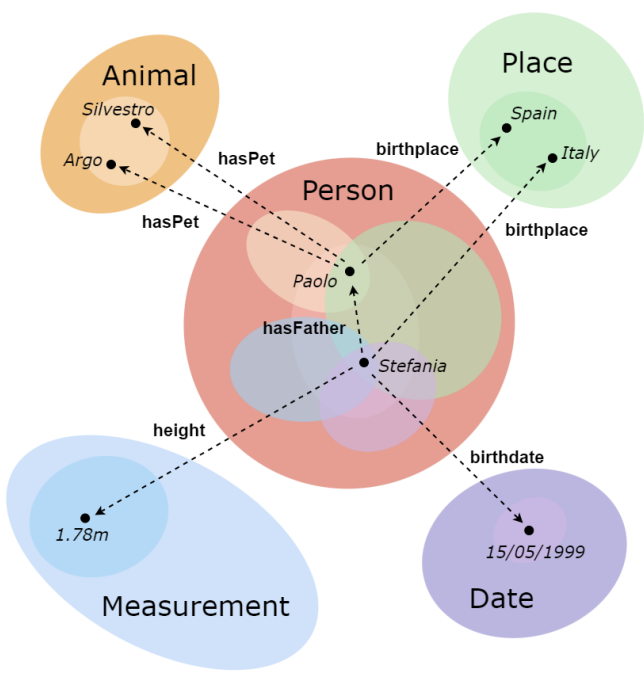
\includegraphics[width=0.7\linewidth]{imgs/img7.1.png}
        \caption{diagramma di Venn di un EG}
    \end{figure}
\end{myobservation}

\begin{myexample}[(Dominio in un \(\hat{\mathcal{EG}}\), Diagramma di Venn)]
    Rappresentiamo i domini degli EG come nella Figura 7.1. Le relazioni sono rappresentate come collegamenti tra entità dell'etipo appropriato e entità o valori dell'etipo o del dtipo appropriato, rispettivamente.
\end{myexample}

\begin{myexample}[(Dominio in \(\hat{\mathcal{ETG}}\), Diagramma di Venn)]
    Rappresentiamo i domini degli ETG come nella Figura 7.1. Le relazioni sono rappresentate come collegamenti tra etipi ed etipi/dtipi.
\end{myexample}

\clearpage
\begin{figure}[ht]
    \centering
    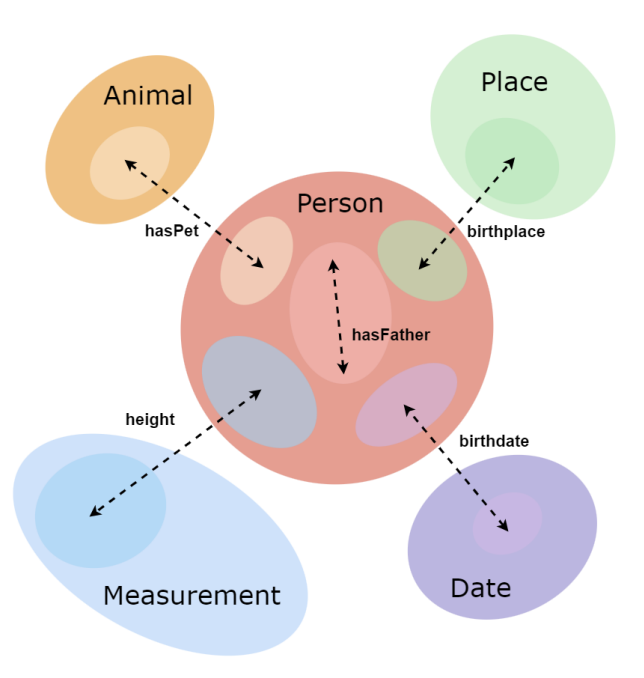
\includegraphics[width=0.7\linewidth]{imgs/img7.2.png}
    \caption{diagramma di Venn di un ETG}
\end{figure}

\section{Linguaggio assertivo}

Sia $\mathcal{L}^i_{\mathcal{KG}} = \mathcal{L}^i_{\mathcal{A}} = \langle \mathcal{E}, \{\mathcal{C}\} \{\mathcal{P}\} \rangle$ lo stencil del $\hat{\mathcal{KG}}$ linguaggio $L^i_{\mathcal{KG}}$. La definizione di $L^i_{\mathcal{KG}}$ segue direttamente dalla definizione di $\verb|D|^i$ nella Sezione 7.1.

\begin{mydefinition}[(Concetto)]
    Abbiamo
    \begin{equation}
        \{\mathcal{C}\} = \mathcal{ET} \cup \mathcal{DT}
    \end{equation}

    dove $\mathcal{ET} = \{\mathcal{E}_\mathcal{T}\}$ e $\mathcal{DT} = \mathcal{D}_\mathcal{T}$ sono rispettivamente (nomi dei) \textbf{etipi} e \textbf{dtipi} in $\hat{\mathcal{KG}}$
\end{mydefinition}

\begin{mydefinition}[(Proprietà degli oggetti e dei dati)]
    \begin{equation}
        \{\mathcal{P}\} = \{\mathcal{OP}\} \cup \{\mathcal{DP}\}
    \end{equation}
    dove $\{\mathcal{OP}\}$ e $\{\mathcal{DP}\}$ sono definiti come segue:
    
    \begin{equation}
        \begin{aligned}
            \{\mathcal{OP}\} \subseteq \{\mathcal{E_T}\} \times \{\mathcal{E_T}\} \\
            \{\mathcal{OP}\} \subseteq \{\mathcal{E_T}\} \times \{\mathcal{E_T}\}
        \end{aligned}
    \end{equation}

    Gli elementi di $\{\mathcal{OP}\}$ sono chiamati proprietà degli oggetti, quelli di $\{\mathcal{DP}\}$ proprietà dei dati.
\end{mydefinition}

\begin{myexample}[(\(\mathcal{EG}\))]
    L'$\mathcal{EG}$ di questo esempio rappresenta il dominio descritto nell'Esempio 7.3. La chiave dell'osservazione sta nel fatto che il numero di nodi corrisponde al numero di entità e valori, mentre il numero di archi corrisponde ai valori di proprietà istanziate. Si noti come i vincoli di cardinalità $n$-a-$m$ consentano agli archi etichettati con la stessa proprietà di uscire dallo stesso nodo di etipi. Si noti anche come i nodi di dati siano e possano essere solo nodi foglia.
\end{myexample}

\begin{figure}[ht]
    \centering
    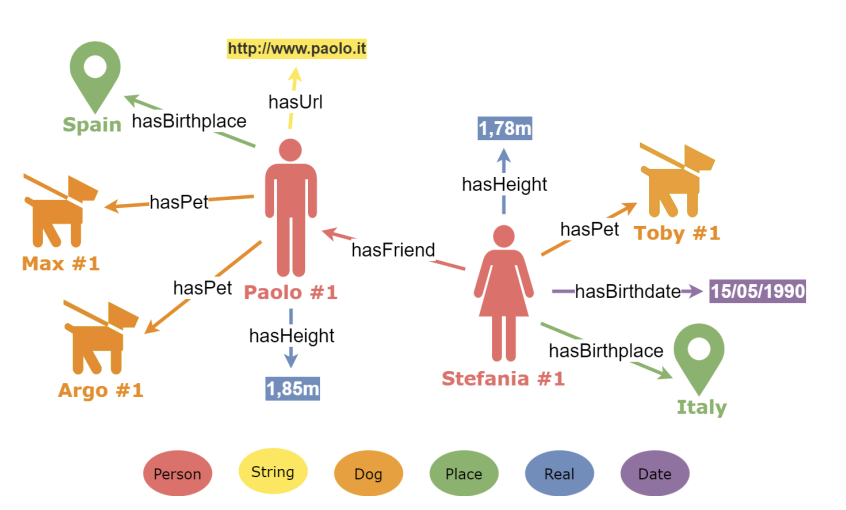
\includegraphics[width=0.7\linewidth]{imgs/img7.3.png}
    \caption{Esempio di un EG che rappresenta informazioni riguardo agli esseri umani.}
\end{figure}


\begin{myexample}[\(\mathcal{ETG}\)]
    L'$\mathcal{ETG}$ di questo esempio rappresenta il dominio descritto nell'Esempio 7.4. C'è un nodo per etipo e tipo di dati. L'$\mathcal{ETG}$ codifica alcune meta-informazioni, ad esempio i vincoli di cardinalità, che possono guidare e controllare la creazione dell'$\mathcal{EG}$ a partire da un $\mathcal{ETG}$. In modo simile agli $\mathcal{EG}$, i nodi dei dtipi sono nodi foglia.
\end{myexample}

\clearpage
\begin{figure}[ht]
    \centering
    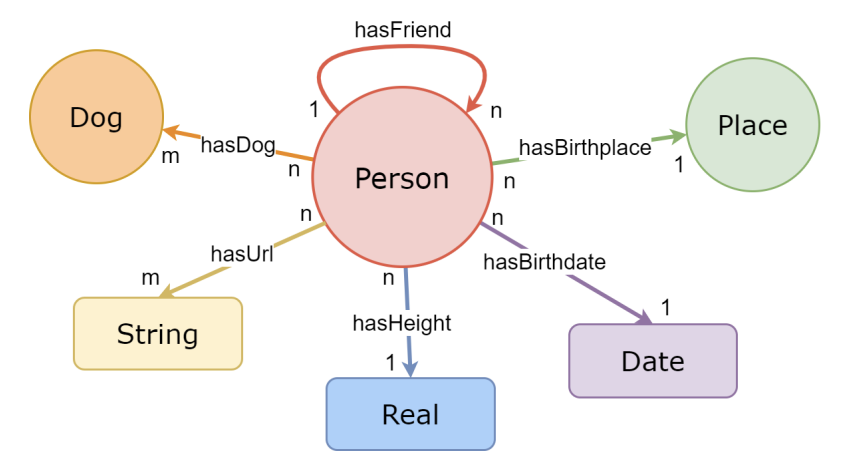
\includegraphics[width=0.7\linewidth]{imgs/img7.4.png}
    \caption{Esempio di un ETG che rappresenta informazioni riguardo agli esseri umani.}
\end{figure}


\begin{myobservation}[(\(\hat{\mathcal{EG}} , \hat{\mathcal{ETG}}, \hat{\mathcal{EEG}} \))]
    Nelle affermazioni di $\hat{\mathcal{KG}}$, le triple sono < nodo, arco, nodo > $\in \mathcal{L}_A$. Nei nodi di $\hat{\mathcal{KG}}$, i nodi $\hat{\mathcal{EG}}$ rappresentano o entità con il loro etipo o valori con il loro dtype. Nei nodi di $\hat{\mathcal{ETG}}$, i nodi rappresentano etipi. Nei nodi di $\hat{\mathcal{EEG}}$, ci sono entrambi i tipi di nodi. Gli archi sono etichettati con nomi di proprietà e rappresentano relazioni. Gli archi da etipi/entità a etipi/entità rappresentano relazioni tra oggetti. Gli archi da etipi/entità a dtipi/valori rappresentano relazioni tra dati.
\end{myobservation}

\section{Funzione di interpretazione}
La funzione di interpretazione di un $\hat{\mathcal{KG}}$ è una mappatura diretta dal linguaggio assertivo $\mathcal{L}^i_{\mathcal{KG}}$ al dominio di interpretazione di destinazione $\verb|D|$. Come si può vedere dagli esempi nella Sezione 7.1 e nella Sezione 7.2, esiste una mappatura quasi diretta tra il linguaggio e il dominio di interpretazione. In pratica, ciò significa che una volta che è stata chiarita la denotazione degli elementi del singolo linguaggio di $\mathcal{L}_{\mathcal{KG}}$ e ci si è assicurati che la funzione di interpretazione soddisfi tutti i requisiti (vedi Sezione 6.4), il significato previsto di un $\mathcal{KG}$ può essere letto direttamente dal $\mathcal{KG}$ stesso.

\section{Grafo di conoscenza}
I modelli di grafo della conoscenza del mondo $\hat{\mathcal{KG}} = \langle \mathcal{L}^i_{\mathcal{KG}}, \verb|D|^i, \mathcal{I}^i_{KG}\rangle $ sono una rappresentazione universale, intuitiva, autoesplicativa ed efficiente dal punto di vista computazionale del mondo.
Una volta fornito un $\hat{\mathcal{KG}}$, è sufficiente per costruire il proprio $\mathcal{KG}$  preferito e tutte le operazioni descritte nella Sezione 6.5 sono disponibili.

\begin{myobservation}[(Tipi di grafi di conoscenza)]
    Come discusso anche nell'Osservazione 6.3, i modelli del mondo e i grafi di conoscenza introdotti finora hanno un'espressività minima. In pratica, i grafi di conoscenza sono spesso arricchiti con ulteriori costruttori che consentono la descrizione di fatti più complessi. Questa è un'operazione del tutto valida con l'avvertenza che è necessario fare attenzione nella selezione del giusto compromesso tra complessità, intuitività e complessità computazionale della rappresentazione selezionata.
\end{myobservation}

\begin{myobservation}[(Dai grafi di conoscenza alla logica)]
    I $\mathcal{KG}$ consentono una facile incorporazione nella logica più appropriata con l'obiettivo di consentire il ragionamento su di essi. Questo sarà l'argomento delle sezioni successive.
\end{myobservation}

\section{Esercizi}

\begin{myexercise}[(Crea un diagramma di insiemi)]
    Considera questa mappa della metropolitana di Milano:
    \begin{figure}[ht]
        \centering
        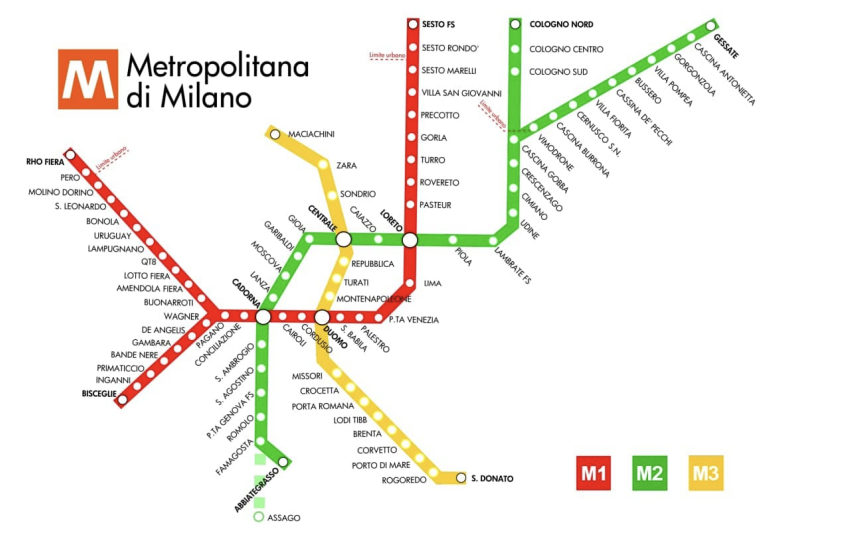
\includegraphics[width=0.7\linewidth]{imgs/img7.5.png}
        \caption{Mappa della metropolitana di Milano}
    \end{figure}

    Cosa deve essere fatto:
    \begin{itemize}
        \item Estrarre insiemi rilevanti di oggetti: Linee, Stazioni, Incroci, Terminali, Numero di stazioni, Colori, ...
        \item Istanziare elementi del dominio: Linea rossa, Cadorna, RHO fiera, Milano, Giallo
        \item Estrarre relazioni rilevanti: haColore, appartieneA, faParteDi, vicinoA, ...
    \end{itemize}
\end{myexercise}

\chapter{Rappresentazione estensionale della logica}

\end{document}